\documentclass{anstrans}
%%%%%%%%%%%%%%%%%%%%%%%%%%%%%%%%%%%
\title{Adjoint-based Sensitivity for Radiation Transport Using an Eddington Tensor Formulation}
\author{Ian Halvic,$^{*}$ Jean Ragusa,$^{*}$}

\institute{
$^{*}$ Texas A\&M University,
College Station, TX, iwhalvic@tamu.edu}


% Optional disclaimer: remove this command to hide
%\disclaimer{Notice: this manuscript is a work of fiction. Any resemblance to
%actual articles, living or dead, is purely coincidental.}

%%%% packages and definitions (optional)
\usepackage{graphicx} % allows inclusion of graphics
\usepackage{booktabs} % nice rules (thick lines) for tables
\usepackage{microtype} % improves typography for PDF
\usepackage{amsmath, amssymb, amsfonts, float, esint, subcaption, xspace, xcolor} 
%\newcommand{\SN}{S$_N$}
%\renewcommand{\vec}[1]{\bm{#1}} %vector is bold italic
%\newcommand{\vd}{\bm{\cdot}} % slightly bold vector dot
%\newcommand{\grad}{\vec{\nabla}} % gradient
%\newcommand{\ud}{\mathop{}\!\mathrm{d}} % upright derivative symbol

\newcommand{\vr}{\vec{r}}
\newcommand{\vp}{\vec{p}}
\newcommand{\vOmega}{\vec{\Omega}}
\newcommand{\vJ}{\vec{J}}
\newcommand{\vO}{\vec{\Omega}}
\newcommand{\bra}{\left\langle}
\newcommand{\ket}{\right\rangle}
\newcommand{\braSN}{\left\langle \! \left\langle}
\newcommand{\ketSN}{\right\rangle \! \right\rangle}
\newcommand{\sbraSN}{\left[ \! \left[}
\newcommand{\sketSN}{\right] \! \right]}
\newcommand{\sbra}{\left[}
\newcommand{\sket}{\right]}
\renewcommand{\div}{\vec{\nabla} \cdot}
\newcommand{\grad}{\vec{\nabla}}
\newcommand{\vbeta}{\vec{\beta} }
\newcommand{\pdx}{\frac{\partial}{\partial x}}
\newcommand{\pdy}{\frac{\partial}{\partial y}}
\newcommand{\pdz}{\frac{\partial}{\partial z}}
\newcommand{\intrrr}{\int d^3 r \,}
\newcommand{\intrr}{\int d^2 r \,}
\newcommand{\dEdphi}{\partial_\phi E }
\newcommand{\dEdp}{\partial_p E }
\newcommand{\dBdphi}{\partial_\phi B }
\newcommand{\dBdp}{B }
\newcommand{\adj}{\phi^\dag}
\newcommand{\vefadj}{\varphi^\dag}
\newcommand{\surf}{\int_{\partial V}}
\newcommand{\domain}{V}
\newcommand{\bound}{\partial V}
\newcommand{\vn}{\vec{n}}
\newcommand{\Edd}{\mathbb{E}}
\newcommand{\BEdd}{B}
\newcommand{\sigt}{\sigma_t}
\newcommand{\sigs}{\sigma_s}
\newcommand{\siga}{\sigma_a}
%\newcommand{\isigt}{\sigma_t^{-1}}
%\newcommand{\isigtp}{\sigma_{t,p}^{-1}}
\newcommand{\isigt}{\ell_t}
\newcommand{\isigtp}{\ell_{t,p}}
\newcommand{\angSource}{\frac{q}{4 \pi}}
\newcommand{\angSourcep}{\frac{q_p}{4 \pi}}
\newcommand{\angSourcepd}{\frac{q_p+\delta q_p}{4 \pi}}
\newcommand{\angSourced}{\frac{\delta q}{4 \pi}}
\newcommand{\scalSource}{q}
\newcommand{\angResp}{q^\dag}
\newcommand{\scalResp}{q^\dag}
\newcommand{\qoi}{{\it QoI}\xspace}


\begin{document}
%%%%%%%%%%%%%%%%%%%%%%%%%%%%%%%%%%%%%%%%%%%%%%%%%%%%%%%%%%%%%%%%%%%%%%%%%%%%%%%%
\section{Introduction}


Adjoint methods are of particular interest for UQ. In general, adjoint methods provide a mechanism for propagating uncertainty and error in the system variables to the uncertainty in the desired quantity of interest (\qoi). This is accomplished in a particularly economical way, sometimes requiring only two differential system solves which can then be used for any combination of sources of error, as opposed to performing an independent solve for each individual error scenario. These adjoint methods have been applied across various complex and time dependent systems. An example of adjoint methods applied to hydrodynamic systems with shocks can be found in Wildey et al. \cite{Wildey}. A more relevant adjoint example to neutron transport occurs in Stripling et al. in the form of reactor burn-up equations \cite{Stripling}.


Application of the adjoint method to transport can pose a major technical limitation. In general, the adjoint method applied to radiation transport requires storing six-dimensional data (the forward angular flux). When dealing with high resolution in these six dimensions, this can potentially require an unreasonable amount of memory for data storage, rendering the method functionally unusable. 

A potential solution to the memory requirement for the transport adjoint formulation is the use of a quasi-diffusion method to reduce the overall dimensionality of the transport problem, from 6D+time to 4D+time. The quasi-diffusion method examined is termed  as a ``Variable Eddington Tensor'' (VET) formulation and uses the unperturbed forward angular flux to compute the Eddington tensor needed in the quasi-diffusion approach. 
%%%%%%%%%%%%%%%%%%%%%%%%%%%%%%%%%%%%%%%%%%%%%%%%%%%%%%%%%%%%%%%%%%%%%%%%%%%%%%%%
\section{Theory}
\subsection{Eddington Formulation and Sensitivity}

In an effort to circumvent the excessive storage requirement for the angular flux, a quasi-diffusive adjoint approach is considered. The approach relies on the Eddington Tensor ($\Edd$) defined as $\Edd \phi = \int d\Omega \vO \vO \psi$ and a Boundary Eddington Factor $B \phi = \int d\Omega \, | \vO \cdot \vn | \psi$ to generate the quasi-diffusive system for a one group steady-state case
\begin{subequations} \label{eqs:EddingtonSystem}
\begin{equation} \label{eq:EddingtonVol}
- \div \left( \isigt(\vr) \div \Edd(\vr) \phi(\vr) \right) + \siga(\vr) \phi(\vr) = \scalSource(\vr) \,,
\end{equation}
inside $\vec{r} \in V$, with boundary condition given by 
\begin{equation} \label{eq:EddingtonBC}
2 J^{\text{inc}}(\vr) = \BEdd(\vr) \phi(\vr) + \vn \cdot \isigt(\vr) \div \Edd(\vr) \phi(\vr)  \quad \vr \in \bound \,.
\end{equation}
\end{subequations}
where $\isigt(\vr)$ denotes the mean free path $\sigt^{-1}(\vr)$. Given the correct value of $\Edd$ from a transport solve, the Eddington System can exactly compute the scalar flux $\phi$, which is sufficient for obtaining quantities of interest in the inner product form $\bra q^\dag , \phi \ket$.

The adjoint system of Eq.~\eqref{eqs:EddingtonSystem} is given as
\begin{subequations}\label{eqs:EddingtonAdjSystem}
\begin{equation}\label{eq:EddingtonAdjVol}
- \Edd : \grad \left( \isigt(\vr) \grad \vefadj \right)  + \siga \vefadj = \scalResp
\end{equation}
\begin{equation}\label{eq:EddingtonAdjBC}
0 = B \vefadj+ \vn \cdot
\Edd \cdot \isigt(\vr) \vec{\nabla} \vefadj    \quad \vr \in \bound
\end{equation}
\end{subequations}

Perturbations are then introduced in the form of $\delta q$, $\delta \siga$, $\delta \sigt$, and $\delta J^{\text{inc}}$ to generate a perturbed system leading to a change in the desired \qoi. Using a first-order perturbation method and making the assumption that $\Edd$ remains unperturbed, the change in the \qoi can be approximated using the inner product
\begin{equation}\label{eqs:sensitivity}
\delta \qoi =  \bra \delta \scalSource - \delta \siga \phi, \vefadj \ket  - \bra \delta \isigt \div \left( \Edd \phi \right) , \grad \vefadj \ket
 + \sbra \vefadj, 2 \delta J^{\text{inc}} \sket \,.
\end{equation}


The proposed method requires an initial solve of the angular transport system to compute $\phi$ and $\Edd$, which are stored for use in Eq.~\eqref{eqs:sensitivity}

Refinements to the VET method are also considered. The first is relatively low cost ``blended'' method which utilizes both the VET and transport adjoint formulations, which selects the most advantageous term for each perturbation. The second is a method of approximating the Eddington perturbation $\delta \Edd$, which relaxes the unperturbed Eddington assumption required for Eq.~\eqref{eqs:sensitivity}.


%\subsection{Eddington Approximation}
%The assumption that $\Edd$ remains unperturbed can cause significant discrepancies in certain systems between the transport and VET found $\delta \qoi$ values. For scenarios where many perturbation cases are to be considered, utilizing additional forward transport solves to characterize the behavior of $\Edd$ under perturbations can offer a refinement of the VET method. A simple linear approximation scheme is tested, in which the parameter of interest $p$ is perturbed by $\delta p$ and a slope of $\Edd$ is found. 
%\begin{equation}
%\label{Eddapprox}
%\frac{\partial \Edd}{\partial p} \approx \frac{\Edd(p+\delta p) - \Edd(p)}{\delta p}
%\end{equation}
%With $\frac{\partial \Edd}{\partial p}$ known an $\delta \Edd$ can then be approximated. An analogous method can then be used to approximate a $\delta \BEdd$ if needed. The sensitivity innter product can then by augmented with $\delta \Edd$ and $\delta \BEdd$ terms to improve accuracy.
%\begin{equation}
%\label{EddErr}
% Eq.~\eqref{eqs:sensitivity}- \bra  \isigt \div \left( \delta \Edd \phi \right), \grad \vefadj \ket
%- \sbra \vefadj, \delta \BEdd \phi \sket \,.
%\end{equation} 



%%%%%%%%%%%%%%%%%%%%%%%%%%%%%%%%%%%%%%%%%%%%%%%%%%%%%%%%%%%%%%%%%%%%%%%%%%%%%%%%
\section{Results}
The approximation of $\delta \qoi$ of various system perturbations using the VET method were tested against the $\delta \qoi$ value found using a transport adjoint method and the ``exact'' $\delta \qoi$ found using the difference of two forward transport solves. The VET system was discretized using a discontinuous finite element method with interior penalty \cite{Arnold}. The transport systems were discretized using an discrete ordinates ($S_n$) solver.

A test case examined is a 1-dimensional 5 section Reed system \cite{ReedProb}, with forward scalar flux solution show in Figure~\ref{fig:Flux4}. Two $\qoi$ values were considered; the first is the average flux in the scatter region $x\in[6,8]$ ($\qoi_5$), the second is the average flux in the central void region $x\in[3,5]$ ($\qoi_3$). The adjoint fluxes resulting from these $\qoi's$ are presented in Figure~\ref{fig:adj}.

Table~\ref{tab:qoi1} and Table~\ref{tab:qoi2} present the $\delta \qoi$ values found using the VET inner-product given in Eq.~\eqref{eqs:sensitivity} and the two refinement methods mentioned.



\begin{figure}
\centering
 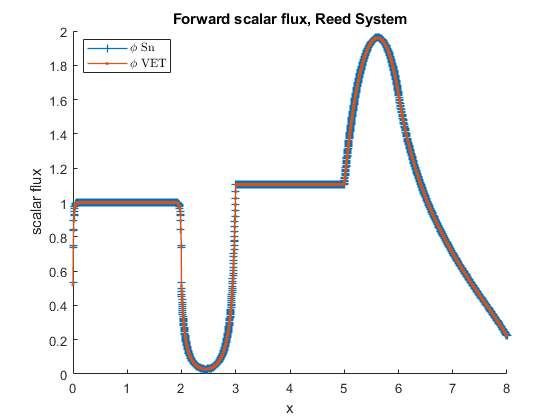
\includegraphics[scale=0.5]{7phi.png}
 \caption{Plot of unperturbed forward scalar flux for the Reed's problem. Flux found using both transport and VET method.}
\label{fig:Flux4}
\end{figure}


\begin{figure}
\centering
\begin{subfigure}{.25\textwidth}
  \centering
  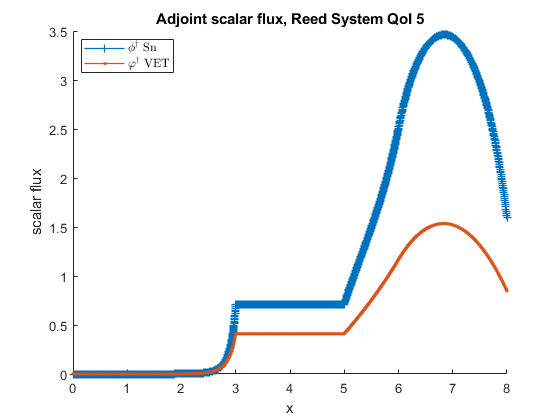
\includegraphics[width=.98\linewidth]{774phia.png}
\end{subfigure}%
\begin{subfigure}{.25\textwidth}
  \centering
  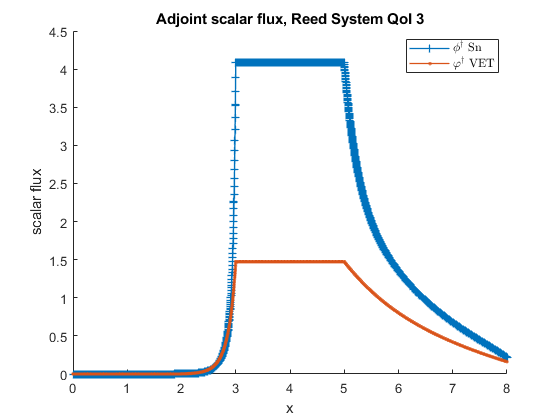
\includegraphics[width=.98\linewidth]{772phia.png}
\end{subfigure}
\caption{Adjoint flux solutions for $\qoi_5$ (left) and $\qoi_3$ (right). Each ha a transport adjoint flux $\phi^\dag$ and a VET adjoint flux $\varphi^\dag$.}
\label{fig:adj}
\end{figure}

\begin{table*}
  \centering
  \caption{$\delta \qoi$ values for $\qoi_5$}
  \begin{tabular}{l|lllll}\toprule
  $\delta\qoi_1$ method    & Exact     & Trans adj     & VET adj      &   VET blended  & VET $\delta \Edd$-appx 
\\ \midrule
$q=+10\%$  & 0.0766009  & 0.0766009  & 0.0765787 & 0.0766009  & 0.0765787
\\
$\siga=+10\%$  &-0.0127845  & -0.0130035 & -0.0130404  & -0.0129986 & -0.0130404
\\
$\sigs=+10\%$  & 0.00856237  & 0.00852152  & 0.00682825  & 0.00682825  & 0.00767834 
\\
$q=+10\%,\siga=+10\%$  & 0.0625379 & 0.0635974  & 0.0635383 & 0.0635604  &  0.0635801 
\\
\bottomrule
\end{tabular}
  \label{tab:qoi1}
\end{table*}


\begin{table*}
  \centering
  \caption{$\delta \qoi$ values for $\qoi_3$}
  \begin{tabular}{l|lllll}\toprule
  $\delta\qoi_2$ method    & Exact     & Trans adj     & VET adj      &   VET blended  & VET $\delta \Edd$-appx 
\\ \midrule
$q=+10\%$  & 0.110511   & 0.110511   & 0.110431 & 0.110511   & 0.110431 
\\
$\siga=+10\%$  &-0.0206607  & -0.0210397 & -0.0202828   & -0.0202828  & -0.0209979
\\
$\sigs=+10\%$  & -0.00953348   & -0.00991779   & 0.00135357   & 0.00135357   & -0.00950217 
\\
$q=+10\%,\siga=+10\%$  & 0.0877841  & 0.0894712   & 0.0901487 & 0.0902281   &  0.0894336  
\\
\bottomrule
\end{tabular}
  \label{tab:qoi2}
\end{table*}



%%%%%%%%%%%%%%%%%%%%%%%%%%%%%%%%%%%%%%%%%%%%%%%%%%%%%%%%%%%%%%%%%%%%%%%%%%%%%%%%
\section{Conclusions}
For the one dimensional systems tested, the VET method preforms reasonably well for estimating $\delta \qoi$ in a  variety of scenarios without needing to store angular flux data. Shortcoming of the VET method when dealing with source perturbations can be partially mitigated using a blended adjoint method combining aspects of the transport adjoint method with the VET. 

With voids present in the system, the unperturbed Eddington approximation can falter when the scattering cross-section is perturbed. By leveraging additional transport solves to characterize the $\delta \Edd$ within the given perturbation space the unperturbed Eddington approximation can be relaxed and a $\delta \Edd$ value can be predicted. This approximation appears to greatly improve the accuracy of the VET formulation in the void scenario

%%%%%%%%%%%%%%%%%%%%%%%%%%%%%%%%%%%%%%%%%%%%%%%%%%%%%%%%%%%%%%%%%%%%%%%%%%%%%%%%
\appendix
%\section{Appendix}

%Inner-products used
%\begin{equation}
%\braSN \psi , f \ketSN  = \int_V dV \int_{4 \pi} d \Omega \,  \psi(\vr, \vO)f(\vr, \vO) \,
%\end{equation}
%\begin{equation}
%\sbraSN \psi , f \sketSN_{\pm}   = \int_{\bound} dS \int_{\vO \cdot \vn \gtrless 0} d\Omega \,  \vO \cdot \vn(\vr) \, \psi(\vr, \vO)f(\vr, \vO) \,
%\end{equation}
%\begin{equation}
%\bra \phi(\vr) , f \ket  = \int_V dV \,  \phi(\vr) g(\vr) \,
%\end{equation}
%\begin{equation}
%\sbra \phi(\vr) , g(\vr)  \sket = \int_{\partial V} dS \, \phi (\vr) g (\vr)  \,
%\end{equation}
%
%\begin{subequations}\label{eqs:TransportSystem}
%\begin{equation}
%\label{SS1GTE}
%\vO \cdot \grad \psi(\vr,\vO) + \sigt(\vr) \psi(\vr,\vO) = \frac{1}{4 \pi} \sigs(\vr) \phi(\vr) + \frac{1}{4 \pi} q(\vr)\, ,
%\end{equation}
%\begin{equation}
%\label{SS1GTE_bc}
%\psi(\vr,\vO) = \psi^{\text{inc}}(\vr,\vO) \quad \vr \in \partial V^{-} = \{ \vr \in \partial V,  \vO \cdot \vec{n}(\vr) < 0\}
%\end{equation}
%\end{subequations}
%\begin{subequations}\label{eqs:TransportAdjSystem}
%\begin{equation}
%\label{SS1GTE}
%- \vO \cdot \grad \psi^\dag(\vr,\vO) + \sigt(\vr) \psi^\dag(\vr,\vO) = \frac{1}{4 \pi} \sigs(\vr) \phi^\dag(\vr) + q^\dag(\vr)\, ,
%\end{equation}
%\begin{equation}
%\label{SS1GTE_bc}
%\psi^\dag(\vr,\vO) = \psi^{\dag,\text{out}}(\vr,\vO) \quad \vr \in \partial V^{+} = \{ \vr \in \partial V,  \vO \cdot \vec{n}(\vr) > 0\}
%\end{equation}
%\end{subequations}
%Sensitivity
%\begin{equation}
%\delta \qoi = \bra \angSourced  + \frac{\delta\sigs}{4 \pi} \phi , \phi^\dag  \ket - \braSN  \delta \sigt \psi , \psi^\dag \ketSN - \sbraSN \delta \psi^{\text{inc}}, \psi^\dag \sketSN_- \,.
%\end{equation}

%%%%%%%%%%%%%%%%%%%%%%%%%%%%%%%%%%%%%%%%%%%%%%%%%%%%%%%%%%%%%%%%%%%%%%%%%%%%%%%%
\section{Acknowledgments}
The work presented here was supported by a graduate assistantship from the U.S. DOE NNSA's PSAAP program (Predictive Science Academic Alliance Program), Grant DE-NA0002376.  

%%%%%%%%%%%%%%%%%%%%%%%%%%%%%%%%%%%%%%%%%%%%%%%%%%%%%%%%%%%%%%%%%%%%%%%%%%%%%%%%
\bibliographystyle{ans}
\bibliography{QoI_MS}
\end{document}

